
\chapter{Biased Random Key Genetic Algorithm}

\section{Algoritmos Genéticos}

Los algoritmos genéticos, o GAs (Genetic Algorithims), \cite{Goldberg} aplican el concepto de supervivencia del más apto para encontrar soluciones óptimas o casi óptimas a los problemas de optimización combinatoria. Se hace una analogía entre una solución y un individuo en una población. Cada individuo tiene un cromosoma correspondiente que codifica la solución. Un cromosoma consiste en una cadena de genes. Cada gen puede tomar un valor, llamado alelo, de algún alfabeto. Los cromosomas tienen asociado a ellos un nivel de condición física que está correlacionado con el correspondiente valor de la función objetivo de la solución que codifica. Los algoritmos genéticos resuelven un conjunto de individuos que forman una población a lo largo de varias generaciones. En cada generación, una nueva población se crea combinando elementos de la población actual para producir hijos que conforman la próxima generación. La mutación aleatoria también tiene lugar en algoritmos genéticos como un medio para escapar de atrapamiento en mínimos locales. El concepto de supervivencia del más apto juega en los algoritmos genéticos cuando los individuos son seleccionados para aparearse y producir descendencia. Los individuos son seleccionados al azar, pero aquellos con mejor estado físico son preferidos sobre aquellos que son menos aptos.

\section{RKGA}

Introducido por Bean \cite{Bean}, en los algoritmos genéticos con claves aleatorias, ó Random Key Genetic Algorithms (RKGA) los cromosomas son representados por un vector de números reales generados aleatoriamente en el intervalo [0, 1]. Un algoritmo determinístico, llamado decodificador, toma como entrada un cromosoma y asocia con ella una solución del problema de optimización combinatoria para el cual se puede calcular un valor objetivo o aptitud física. Los algoritmos RKGAs evolucionan una población de vectores de claves aleatorios sobre una serie de iteraciones llamadas generaciones. La población inicial se compone de $p$ vectores de claves aleatorias. Cada alelo se genera independientemente al azar en el intervalo real [0, 1]. Después de calcular la aptitud de cada individuo por el decodificador, la población se divide en dos grupos de individuos. Un pequeño grupo de individuos de élite $p_e$, es decir, aquellos con mejores valores de aptitud individual. El segundo el conjunto remanente de $p-p_e$ no elite individuos donde $p_e<p-p_e$. Con el fin de evolucionar a la población, un RKGA utiliza una estrategia elitista ya que todos los individuos de élite de la generación $k$ se copian sin cambios a la generación $k + 1$. Esta estrategia mantiene un seguimiento de las buenas soluciones encontradas durante las iteraciones del algoritmo que resulta en una heurística de mejora monotónica. La mutación se utiliza para permitir que los GAs escapen de la trampa en mínimos locales. En RKGA un mutante es un individuo generado a partir de un vector de claves aleatorias, de la misma manera que un elemento de la población inicial. Con la poblacion $p_e$ elite y la $p_m$ mutantes, un conjunto adicional de individuos $p - p_e - p_m$ es requerido para completar la generacion $k+1$. Esto se hace generando una descendencia mediante el proceso de apareamiento.

\section{BRKGA}\label{sec:brkga}

En RKGA, Bean \cite{Bean} selecciona dos padres al azar de toda la población. Un BRKGA (Biased Random Key Genetic Algorithms), difiere de RKGA en la forma en que los padres son seleccionados para el apareamiento. En un BRKGA, cada elemento se genera combinando un elemento seleccionado al azar de la partición de elite en la población actual y uno de la partición no elitista. En algunos casos, el segundo padre se selecciona de toda la población. Se permite la repetición en la selección de un padre y, por lo tanto, un individuo puede producir más de un hijo. Como $p_e < p - p_e$, la probabilidad de que un individuo de élite sea seleccionado para el apareamiento es mayor que la de un individuo no élite y por lo tanto un individuo de élite tiene un mayor probabilidad de transmitir sus genes a generaciones futuras. Otro factor que contribuye a este fin es el crossover uniforme parametrizado (Spears y DeJong \cite{SpearsDeJong}), el mecanismo utilizado para implementar el apareamiento en BRKGAs. Sea $\rho_e > 0,5$ la probabilidad de que un descendiente herede el alelo de su padre de elite. Sea $n$ el número de cromosomas de un individuo, para $i =1,...,n$ el i-ésimo alelo $c_i$ del descendiente $c$, este alelo $c_i$ toma el valor del i-ésimo alelo $e_i$ del padre de elite $e$ con una probabilidad $p_e$ y el valor del $e'_i$ del padre no elite con probabilidad $1-p_e$. Este proceso se puede ver en la figura \ref{fig:biasCrossover}. De esta manera, es más probable que la descendencia herede características del padre de élite que las del padre no de élite. Dado que asumimos que cualquier vector de clave aleatoria puede ser decodificado en una solución, entonces el descendiente de apareamiento es siempre válido, es decir, puede ser decodificado en una solución del problema de optimización combinatoria.

\begin{figure}[h]
	\caption{Bias crossover}
	\centering
	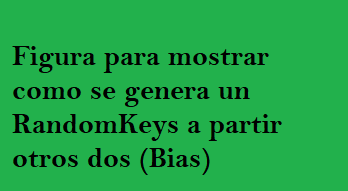
\includegraphics{BiasCrossover}
	\label{fig:biasCrossover}
\end{figure}

\bigskip

En la figura \ref{fig:evolucion} se puede observar como la evolución funciona. Los individuos son ordenados por su aptitud y marcados como elite y no-elite. Los vectores aleatorios de elite y pasan directamente a la siguiente generación. Un porcentage pequeño de la nueva generacion sera conformado por individuos mutantes, generados aleatoriamente como la poblacion inicial. Por último, el último conjunto de la nueva población se crean del cruce entre individuos de la población de elite con individuos de la población no-elite. En la figura el primer vector de cromosomas es de un individuo de elite, el segundo vector de cromosomas es de un edividuo no-elite. Se decide que cromosomas tomara el individuo hijo utilizando un vector aleatorio del mismo tamaño que los vectores de cromosmos. En este ejemplo se utiliza un $\rho_e = 0.70$, de este modo la descendencia se asemejara mas al padre de elite. Con estos cruces se completa la nueva generación de soluciones.

\begin{figure}[h]
	\caption{Evolución de una población}
	\centering
	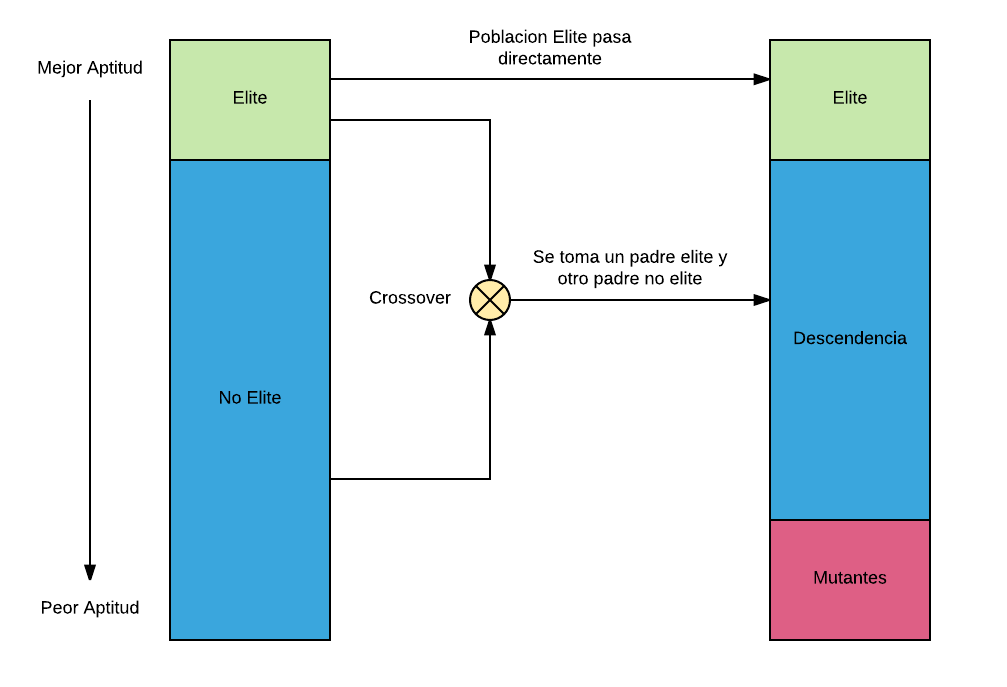
\includegraphics{EvolucionPoblacion}
	\label{fig:evolucion}
\end{figure}

\section{Decodificador del BRKGA}

Una caracterisitca importante para mencionar del BRKGA es que que el decodificador es el único modulo del algoritmo que requiere conocimiento del dominio del problema. El decodificador transforma un vector aleatorio de enteros en una instancia de una solución del problema. Es un adaptador, por lo tanto si hacemos un decodificador para otro problema podríamos reutilizar el modulo de BRKGA.

\bigskip

En el caso de mi impementación del BRKGA entre cada generación se ejecutan unas heuristicas de busqueda local sobre las mejores soluciones de la población. Como estas heuristicas trabajan sobre una instancia de la solución, requiere que exista un objeto codificador. Es decir, es decir un algoritmo capas de convertir una solución del problem en un vector de enteros aleatorios. De este modo, una vez que se mejora una solución, podemos actualizar su vector aleatorio que lo representa y seguir el curso del BRKGA. 

